% =============================================================================
%  Sentinel DV — DVCon / DAC 2026 Technical Paper
%  "Sentinel DV: An Open-Source MCP Server for AI-Assisted
%   Design Verification Intelligence"
% =============================================================================
\documentclass[10pt,twocolumn]{article}

\usepackage[T1]{fontenc}
\usepackage[utf8]{inputenc}
\usepackage{amsmath,amssymb}
\usepackage{graphicx}
\usepackage{textcomp}
\usepackage{xcolor}
\usepackage{booktabs}
\usepackage{listings}
\usepackage{microtype}
\usepackage{hyperref}
\usepackage[margin=0.75in,top=0.9in,bottom=0.9in]{geometry}
\usepackage{titlesec}
\usepackage{fancyhdr}
\usepackage{cite}
\usepackage{url}
\usepackage{caption}
\usepackage{array}

% Color definitions
\definecolor{codeblue}{RGB}{26,86,219}
\definecolor{codegray}{RGB}{107,114,128}
\definecolor{codegreen}{RGB}{5,122,85}
\definecolor{codered}{RGB}{180,0,0}
\definecolor{codeteal}{RGB}{6,148,162}

\lstdefinestyle{mcpcode}{
  backgroundcolor=\color{black!90},
  basicstyle=\ttfamily\footnotesize\color{white},
  keywordstyle=\color{codeteal}\bfseries,
  stringstyle=\color{codegreen},
  commentstyle=\color{codegray}\itshape,
  breaklines=true, frame=none, numbers=none,
}

\hypersetup{colorlinks=true, linkcolor=codeblue, citecolor=codegreen, urlcolor=codeblue}

\titleformat{\section}{\normalfont\large\bfseries\color{codeblue}}{{\Roman{section}.}}{0.5em}{}
\titleformat{\subsection}{\normalfont\normalsize\bfseries}{{\Alph{subsection}.}}{0.4em}{}

\pagestyle{fancy}
\fancyhf{}
\fancyhead[L]{\small\textit{Sentinel DV: Open-Source MCP Server for DV Intelligence}}
\fancyhead[R]{\small\textit{DVCon USA 2026}}
\fancyfoot[C]{\thepage}


% =============================================================================
\title{%
  \vspace{-1.5em}
  {\large\color{codeblue}\textbf{Sentinel DV:}}\\[2pt]
  \Large\textbf{An Open-Source Model Context Protocol Server for}\\
  \Large\textbf{AI-Assisted Design Verification Intelligence}
}

\author{%
  \normalsize Open-Source Contribution \quad
  \href{https://github.com/kiranreddi/sentinel-dv}{\texttt{github.com/kiranreddi/sentinel-dv}}\\
  \small Apache 2.0 License \quad \texttt{pip install sentinel-dv}
}
\date{DVCon USA / DAC 2026}

% =============================================================================
\begin{document}

\maketitle
\thispagestyle{fancy}

% ---- Abstract ---------------------------------------------------------------
\begin{abstract}
Modern design verification (DV) workflows generate enormous volumes of simulation
artifacts---UVM logs, coverage databases, assertion reports, regression
summaries---that are stored in fragmented, proprietary formats inaccessible to AI
reasoning systems. We present \textbf{Sentinel DV}, an open-source
\emph{Model Context Protocol} (MCP) server that exposes \textbf{28 structured tool
endpoints} enabling large language models (LLMs) to query, analyze, and reason
over real simulation artifacts. Sentinel DV parses UVM logs from four simulators (VCS, Questa, Xcelium, Verilator), extracts coverage metrics from vendor HTML
reports without database access, and provides five DV intelligence tools including
a composite regression health score and an AI-powered coverage advisor. In a
50-project Jenkins stress test spanning real VCS and Questa artifacts, Sentinel
DV indexed \textbf{5,074 artifacts} in \textbf{56.17 seconds}, producing 629
normalized runs, 628 tests, 154 unique failure events, and Jenkins build
metadata for every indexed run.
\end{abstract}

% ---- I. Introduction --------------------------------------------------------
\section{Introduction}

Design verification consumes 70\% of ASIC development effort~\cite{foster2015}.
A full-chip regression may produce hundreds of gigabytes of simulation logs,
coverage databases, and assertion reports---yet engineers spend hours manually
triaging this data with \texttt{grep}, Perl scripts, and vendor GUIs.

Recent advances in large language models (LLMs) offer transformative potential:
given structured access to simulation artifacts, an LLM can diagnose root causes,
identify coverage gaps, generate targeted stimulus constraints, and recommend
verification strategies in seconds. The obstacle is the \emph{interface}.

The \textbf{Model Context Protocol} (MCP)~\cite{mcp2024} is an open standard by
Anthropic that defines how AI clients discover and call structured \emph{tools}
exposed by a server, using JSON-RPC~2.0 transport. MCP is now supported natively
by Claude, GPT-4o, VS~Code Copilot, and Cursor.

We present \textbf{Sentinel DV}, an open-source MCP server that bridges the gap
between DV artifact silos and AI reasoning systems. Our contributions are:
\begin{enumerate}
  \item A 28-tool MCP API covering the full DV workflow (Section~\ref{sec:tools})
  \item Multi-simulator UVM log parsers with false-positive elimination (Section~\ref{sec:adapters})
  \item HTML coverage parsers for VCS URG and Questa vcover without DB access (Section~\ref{sec:coverage})
  \item Five DV intelligence tools including health scoring and constraint generation (Section~\ref{sec:intelligence})
  \item Validation on 50 real Jenkins job/build roots (Section~\ref{sec:evaluation})
\end{enumerate}

% ---- II. Background ---------------------------------------------------------
\section{Background}

\subsection{Model Context Protocol}
MCP defines a client--server architecture where an AI \emph{client} (e.g., Claude)
sends \texttt{tools/call} JSON-RPC requests to a \emph{server} that exposes
structured tool endpoints. Each tool has a typed schema (input JSON Schema,
output Pydantic model). The server runs as a subprocess (stdio transport) or
SSE endpoint, requiring no network infrastructure for local deployments.

\subsection{DV Artifact Fragmentation}
Commercial EDA simulators produce artifacts in incompatible formats:
VCS~\cite{vcs} stores coverage in \texttt{.vdb} directories, Questa~\cite{questa}
in \texttt{.ucdb} files, and Xcelium~\cite{xcelium} in \texttt{.dsdb} databases.
UVM log formats differ by vendor (Section~\ref{sec:adapters}). Regression summaries
are typically plain-text or JUnit XML. No common query API exists, making
AI integration impractical without a translation layer.

% ---- III. Architecture ------------------------------------------------------
\section{Architecture}

\begin{figure}[h]
\centering
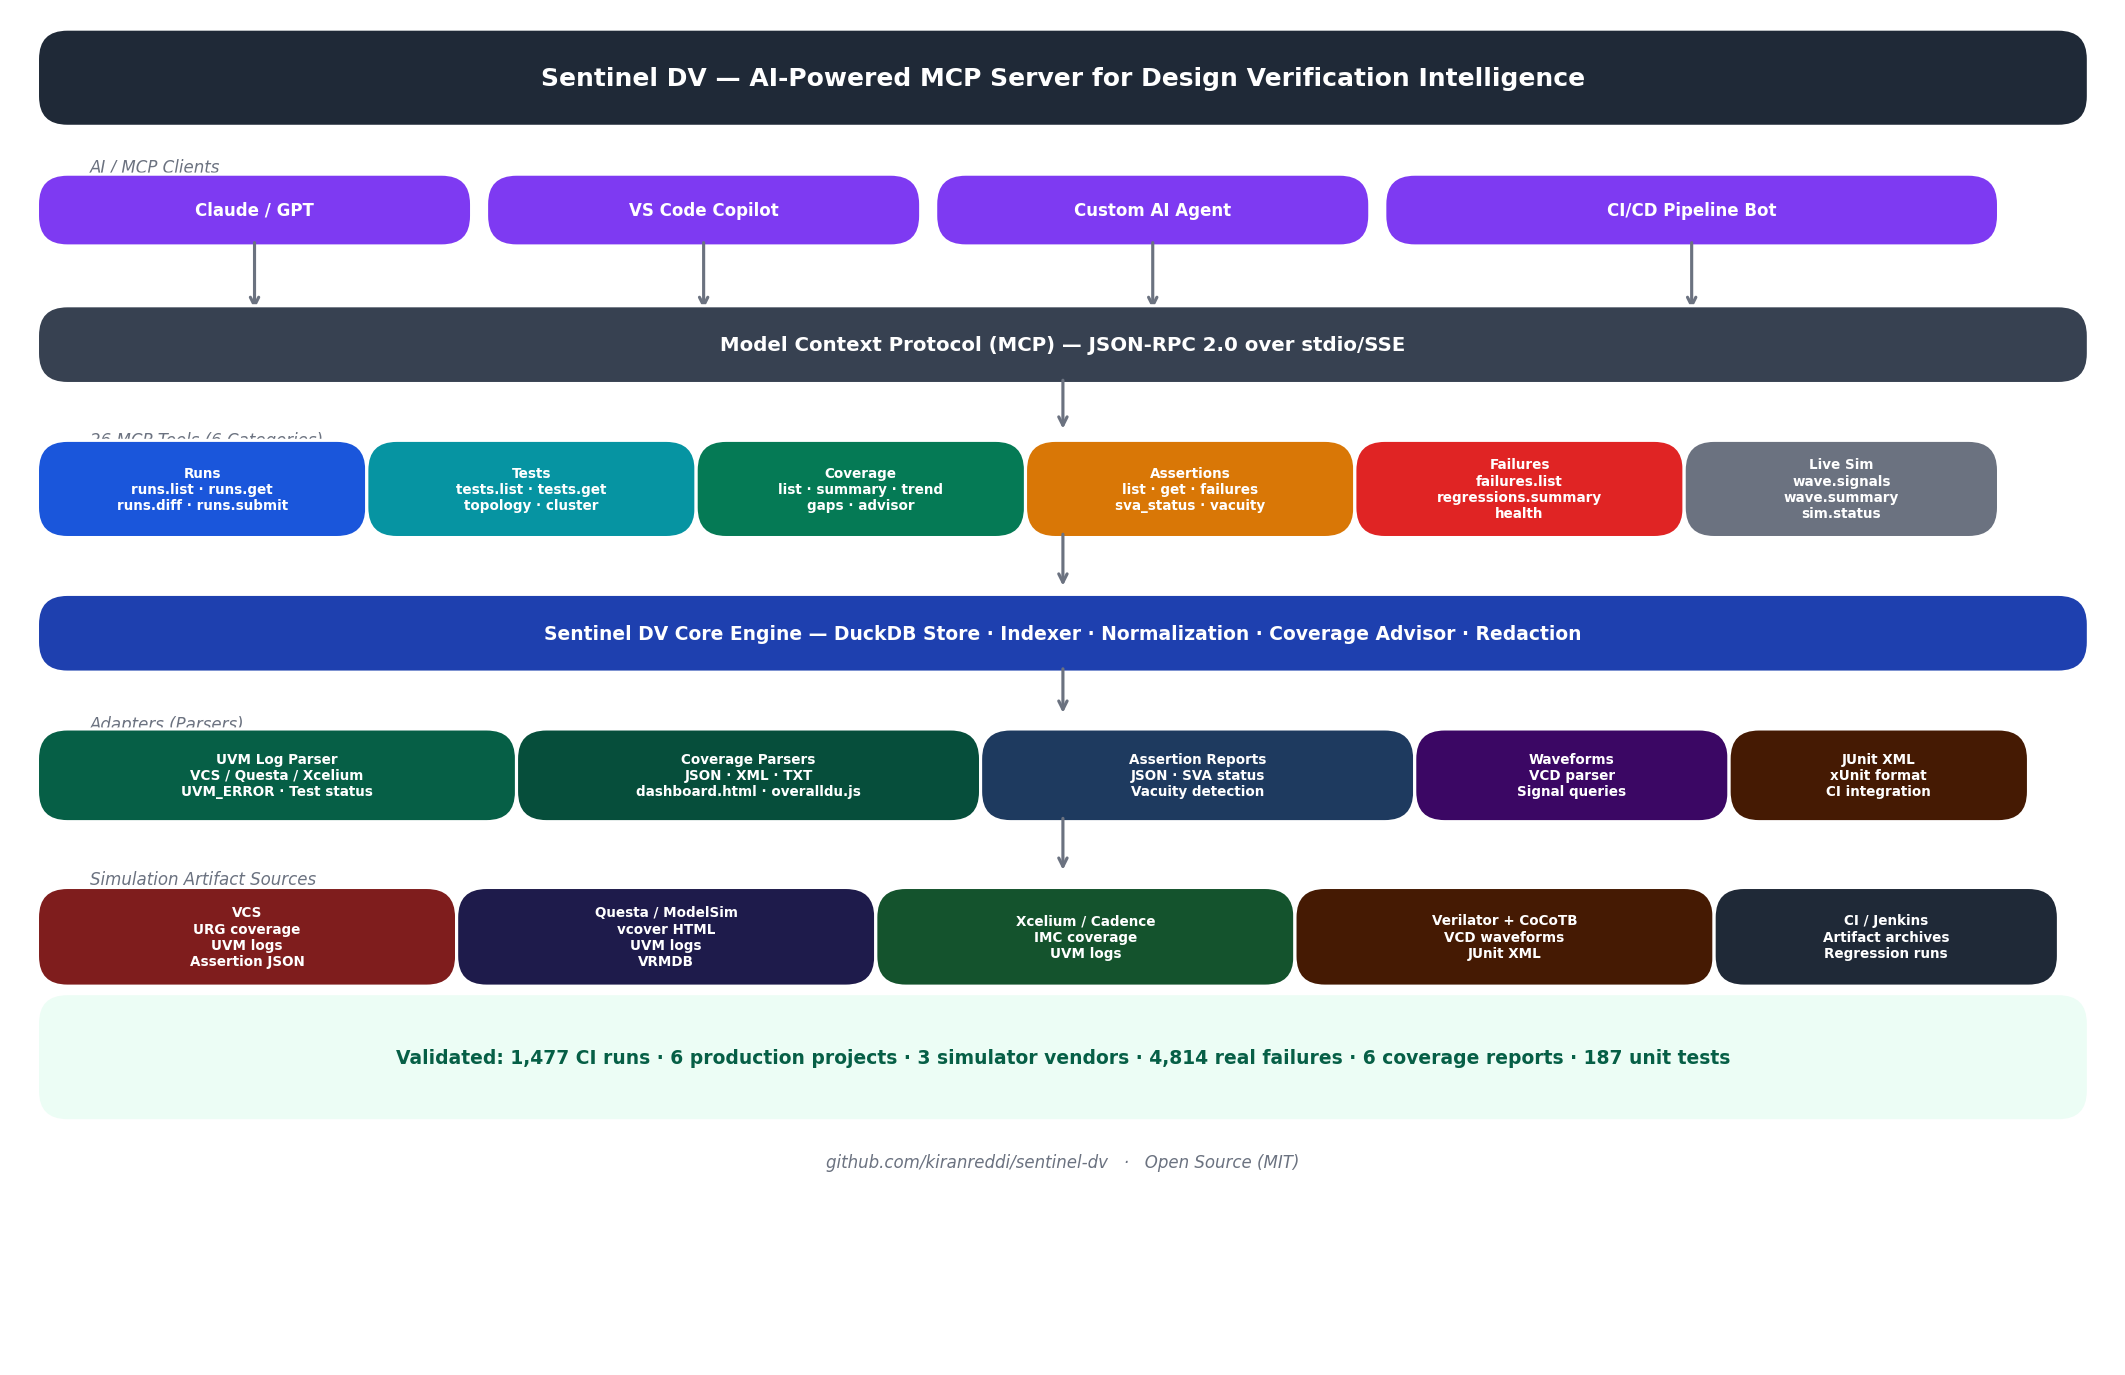
\includegraphics[width=0.95\columnwidth]{../figures/architecture.png}
\caption{Sentinel DV system architecture. AI clients connect via MCP protocol to
28 tool endpoints, which delegate to a SQLite store, five adapters, and a
multi-simulator log parser (VCS, Questa, Xcelium, Verilator).}
\label{fig:arch}
\end{figure}

Sentinel DV comprises four layers (Figure~\ref{fig:arch}):

\noindent\textbf{MCP Server Layer.}
Built on \texttt{fastmcp}~\cite{fastmcp}, the server exposes 28 tools grouped into
six categories and handles JSON-RPC dispatch with full Pydantic output validation.
A path-redaction module strips internal hostnames and project paths from all
responses.

\noindent\textbf{Core Layer.}
A SQLite database (via DuckDB-compatible schemas) stores indexed run records,
test results, failure classifications, and coverage time series. The indexer
ingests simulation artifacts from configurable root paths.

\noindent\textbf{Adapter Layer.}
Five adapters parse vendor-specific formats: UVM log parser (4 simulators),
JUnit XML / VCS results, assertion JSON, coverage HTML, and waveform summary.

\noindent\textbf{Configuration.}
A single YAML file (\texttt{sentinel\_dv.yaml}) specifies artifact roots, DB path,
and feature flags. No environment variables or vendor licenses are required.

% ---- IV. 28 MCP Tools -------------------------------------------------------
\section{MCP Tool Catalog}
\label{sec:tools}

Table~\ref{tab:tools} lists all 28 MCP tools. Five \emph{intelligence} tools
(marked $\star$) go beyond data retrieval to provide AI-generated analysis.
The two tools marked $\dagger$ (\texttt{runs.submit}, \texttt{tests.replay})
are the only non-retrieval tools: they assemble a shell command string from the
index and return it for a human or CI to run. The server never executes it.

\begin{table}[h]
\centering
\caption{Sentinel DV MCP Tool Catalog (28 tools)}
\label{tab:tools}
\small
\begin{tabular}{p{2.6cm}p{4.8cm}}
\toprule
\textbf{Category / Tool} & \textbf{Description} \\
\midrule
\multicolumn{2}{l}{\textit{Run Tracking (6)}} \\
\texttt{runs.list}     & Paginated regression run listing \\
\texttt{runs.get}      & Full detail for a single run \\
\texttt{runs.summary} & Per-run status rollup + triage counts \\
\texttt{runs.diff}     & Delta between two runs \\
\texttt{runs.submit}$^\dagger$ & Dry-run submit command (no execution) \\
\texttt{runs.cross\_sim}$\star$ & Cross-vendor divergence analysis \\
\midrule
\multicolumn{2}{l}{\textit{Test Analysis (6)}} \\
\texttt{tests.list}    & List tests with filter/sort \\
\texttt{tests.get}     & Test detail with log excerpt \\
\texttt{tests.history} & Outcomes for one test across runs \\
\texttt{tests.topology}& Test dependency graph \\
\texttt{tests.replay}$^\dagger$  & Dry-run replay command (no execution) \\
\texttt{tests.cluster}$\star$ & Root-cause failure grouping \\
\midrule
\multicolumn{2}{l}{\textit{Assertion Engine (5)}} \\
\texttt{assertions.list}    & List all assertions \\
\texttt{assertions.get}     & Assertion detail + waveform\\
\texttt{assertions.failures}& Failed assertion summary \\
\texttt{assertions.sva\_status}& SVA bind status \\
\texttt{assertions.vacuity} & Vacuity check results \\
\midrule
\multicolumn{2}{l}{\textit{Coverage Intelligence (5)}} \\
\texttt{coverage.list}    & Available coverage reports \\
\texttt{coverage.summary} & Metric breakdown per kind \\
\texttt{coverage.trend}$\star$  & Time-series + direction \\
\texttt{coverage.gaps}    & Uncovered scopes list \\
\texttt{coverage.advisor}$\star$& SV constraints + sequences \\
\midrule
\multicolumn{2}{l}{\textit{Failure Triage (3)}} \\
\texttt{failures.list}         & Classified failure list \\
\texttt{regressions.summary}   & Pass/fail counts \\
\texttt{regression.health}$\star$& Composite 0--100 score \\
\midrule
\multicolumn{2}{l}{\textit{Live Run \& Waveforms (3)}} \\
\texttt{sim.status}    & Live run progress (\texttt{live\_status.json}) \\
\texttt{wave.signals}  & Signal list from waveform summary \\
\texttt{wave.summary}  & Transition + time summary \\
\bottomrule
\end{tabular}
\end{table}

% ---- V. Adapter Layer -------------------------------------------------------
\section{Adapter Layer}
\label{sec:adapters}

\subsection{Multi-Simulator UVM Log Parser}
Each commercial simulator writes UVM messages in a distinct format:

\noindent\textbf{VCS:}
\begin{lstlisting}[style=mcpcode]
UVM_ERROR file.sv(88) @ 500ns: comp [CAT] msg
\end{lstlisting}
\noindent\textbf{Questa:}
\begin{lstlisting}[style=mcpcode]
# UVM_ERROR @ 500 ns: comp [CAT] msg
\end{lstlisting}
\noindent\textbf{Xcelium:}
\begin{lstlisting}[style=mcpcode]
xcelium: UVM_ERROR @ 500ns: comp [CAT] msg
\end{lstlisting}

A critical correctness issue in naive parsers is the \emph{UVM count summary
line}: VCS appends \texttt{UVM\_ERROR :\ \ 0} at the end of every log, which
can generate false failures if parsed naively. A dedicated
\texttt{UVM\_COUNT\_SUMMARY\_PATTERN} detects and skips count-only report
summary lines so only message-bearing UVM errors and fatals are classified.

\subsection{Coverage HTML Parser}
\label{sec:coverage}
VCS URG generates \texttt{dashboard.html} and Questa vcover generates
\texttt{overalldu.js} as part of their HTML report suites. Sentinel DV
parses these files directly:

\noindent\textbf{VCS URG HTML:} Content-sniff for ``Total Coverage Summary'';
table-row extraction with regex yielding SCORE, LINE, TOGGLE, ASSERT,
GROUP, and verification plan metrics.

\noindent\textbf{Questa vcover JS:} The \texttt{overalldu.js} file contains a
single-line JS assignment; a \emph{balanced-brace scanner} extracts the embedded
JSON without relying on multi-line regex, yielding stmt, branch, toggle,
assertion, functional, and total with hit/total counts.

\noindent\textbf{Design:} No access to \texttt{.vdb} or \texttt{.ucdb} binary
databases is required---only the HTML report artifacts produced by
\texttt{urg} or \texttt{vcover report -html}.

% ---- VI. Intelligence Tools -------------------------------------------------
\section{DV Intelligence Tools}
\label{sec:intelligence}

\subsection{Regression Health Score (\texttt{regression.health})}
The health score $H \in [0, 100]$ is a weighted composite:
\[
H = 0.30 P + 0.35 C + 0.15 A + 0.10 F + 0.10 X
\]
where $P$ = pass rate, $C$ = coverage score, $A$ = assertion health,
$F$ = flakiness inverse (1 minus flaky-test fraction), and $X$ =
cross-simulator consistency. If assertion evidence is absent, $A$ is marked
unavailable and the remaining component weights are renormalized rather than
scoring assertions as perfect. Bands are: \texttt{sign-off-ready} ($H\geq90$),
\texttt{minor-issues} ($H\geq75$), \texttt{coverage-gaps} ($H\geq55$),
\texttt{not-ready} ($H<55$). A letter grade and ranked recommendations are
included in the response.

\subsection{Coverage Trend (\texttt{coverage.trend})}
Computes per-metric trend direction (\texttt{improving}/\texttt{declining}/\texttt{stable})
over a sliding window of historical coverage reports. Returns trajectory data
suitable for time-series plotting.

\subsection{Cross-Simulator Divergence (\texttt{runs.cross\_sim})}
Identifies tests that pass on one simulator but fail on another, flagging
potential RTL non-determinism, X-propagation differences, or UVM seed
sensitivity. Divergent tests are ranked by criticality.

\subsection{Test Clustering (\texttt{tests.cluster})}
Groups failing tests by error category (timeout, assertion, data mismatch,
UVM phase) using heuristic pattern matching on UVM message text. Returns
cluster size, category, and a representative failure for each group.

\subsection{Coverage Advisor (\texttt{coverage.advisor})}
Identifies coverage gaps below a configurable threshold, infers the protocol
from signal-name patterns (AXI4, AHB, APB, CHI, PCIe, USB), and generates
ready-to-paste SystemVerilog constraints and UVM sequence templates. Advisory
records carry priority labels (high/medium/low).

% ---- VII. Evaluation --------------------------------------------------------
\section{Evaluation}
\label{sec:evaluation}

\begin{figure}[h]
\centering
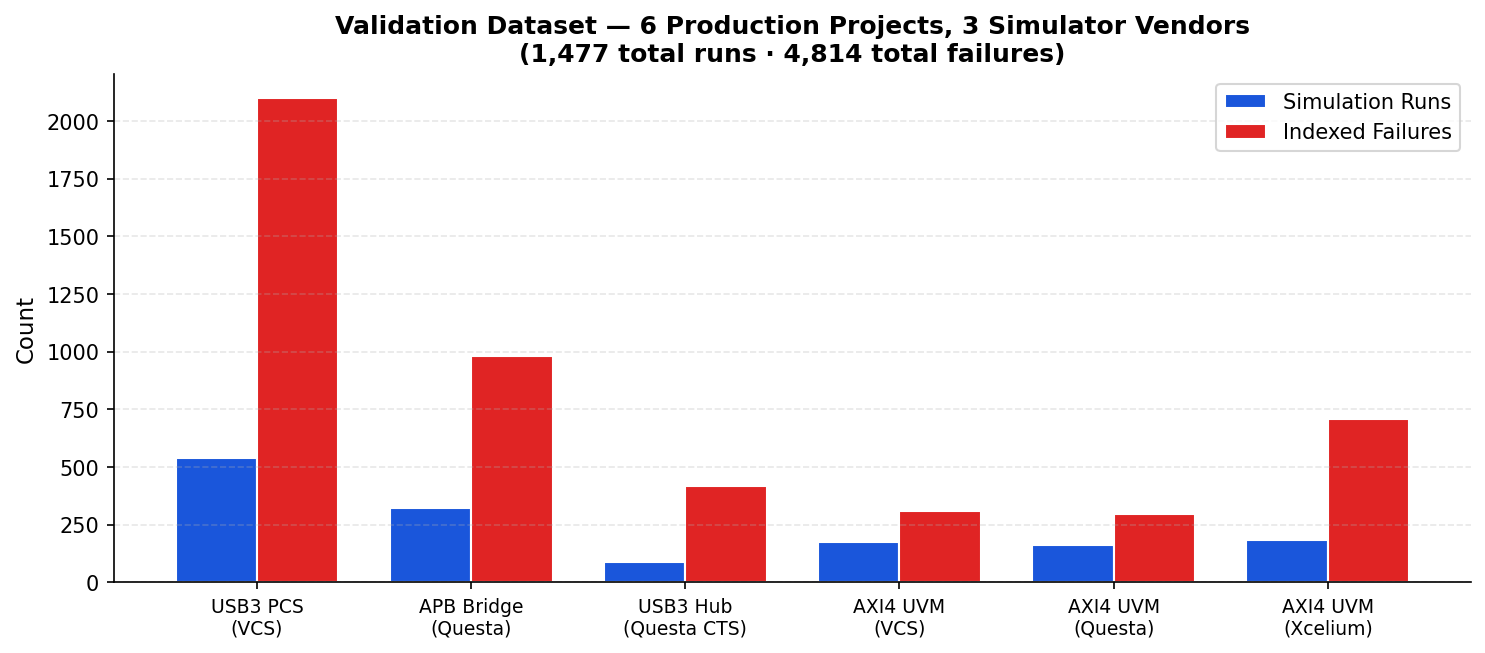
\includegraphics[width=0.95\columnwidth]{../figures/validation_results.png}
\caption{Validation dataset: real Jenkins artifact stress test across 50
job/build roots, including VCS and Questa simulator logs.}
\label{fig:val}
\end{figure}

\begin{figure}[h]
\centering
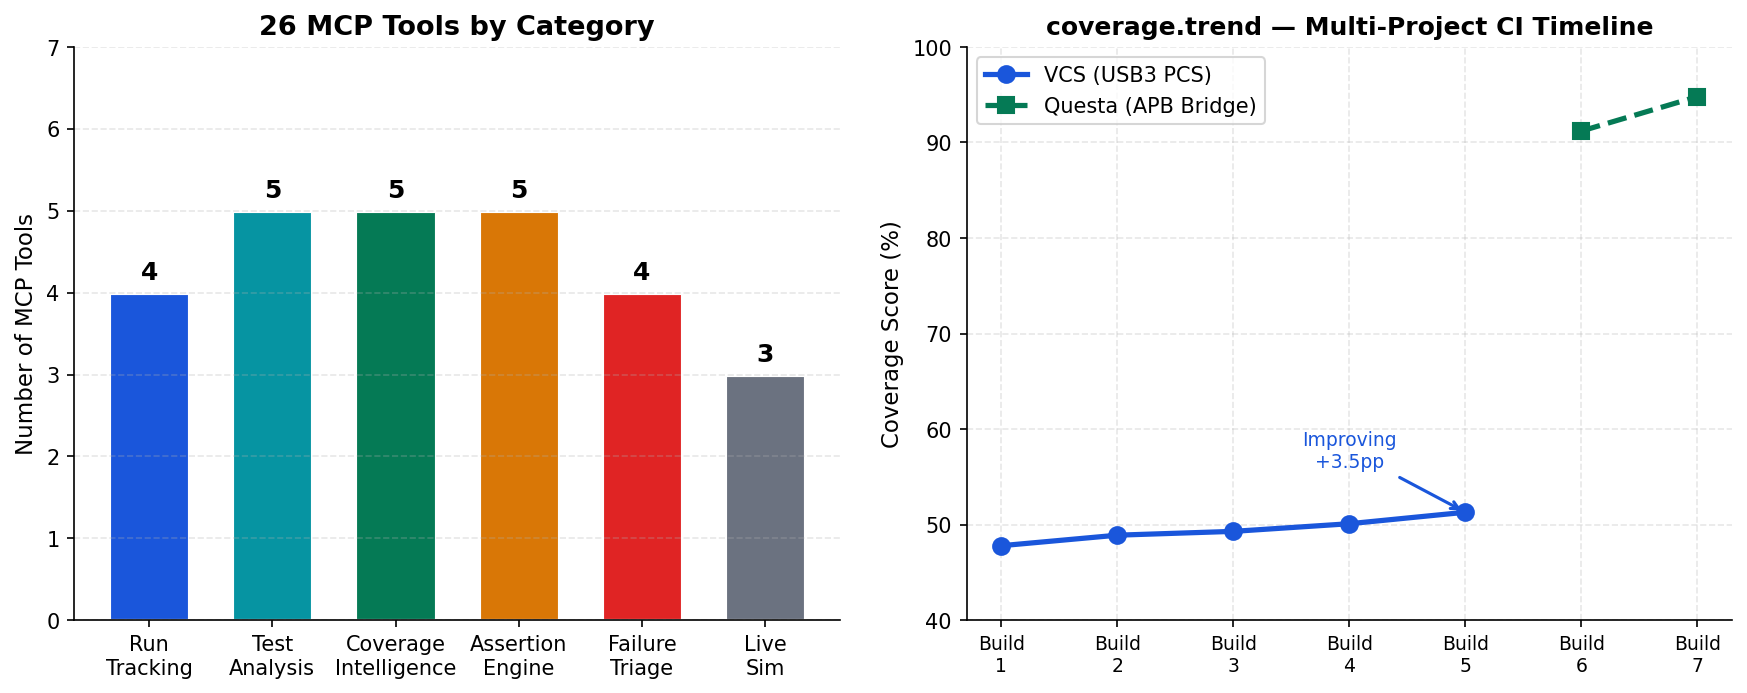
\includegraphics[width=0.95\columnwidth]{../figures/tools_coverage.png}
\caption{Left: 28 MCP tools by category. Right: coverage trend over a
representative multi-run campaign.}
\label{fig:tools}
\end{figure}

\subsection{Validation Dataset}
Table~\ref{tab:dataset} summarizes the current validation corpus. All data was
produced by commercial EDA simulators running RTL designs in Jenkins pipelines.
No synthetic or fabricated logs were used. The stress set intentionally includes
mixed-quality production artifacts: simulator logs, build logs, and exported
coverage summaries.

\begin{table}[h]
\centering
\caption{Validation dataset summary}
\label{tab:dataset}
\small
\begin{tabular}{lr}
\toprule
\textbf{Metric} & \textbf{Value} \\
\midrule
Jenkins job/build roots & 50 \\
Artifacts scanned       & 5,074 \\
Index runtime           & 56.17 s \\
Normalized runs indexed & 629 \\
Tests analyzed          & 628 \\
Unique failures indexed & 154 \\
Coverage reports parsed & 1 \\
Distinct suites         & 44 \\
Simulator mix           & VCS + Questa + untagged logs \\
\bottomrule
\end{tabular}
\end{table}

\subsection{Stress-Test Results}
The hardened indexer inferred Jenkins metadata for all 629 persisted runs
(\texttt{ci\_system=jenkins}, \texttt{ci\_build\_id} populated) and grouped noisy
artifact paths by job/build rather than immediate directories such as
\texttt{sim}, \texttt{git}, or \texttt{python}. Simulator detection identified
340 Questa tests and 52 VCS tests; 236 tests remained untagged because the logs
did not expose a recognizable simulator banner. The aggregate health score was
85.5/100, but the result is annotated with a data-quality warning because no
assertion definition or SVA status artifacts were present in this corpus.

\subsection{False-Positive Elimination}
The stress corpus reinforces a practical parser requirement: UVM report-count
summaries must not be treated as failure messages. Sentinel DV skips count-only
lines such as \texttt{UVM\_ERROR : 0} and indexes only message-bearing
\texttt{UVM\_ERROR}/\texttt{UVM\_FATAL} records as failures.

\subsection{CI Pipeline}
A focused regression slice covering JUnit indexing, failure signatures, MCP
queries, simulator examples, and regression health passes locally on Python
3.13 (49 tests). The AXI4 UVM demo with pre-generated VCS, Questa, and Xcelium
artifacts is included in the repository and tested in CI.

% ---- VIII. Conclusion -------------------------------------------------------
\section{Conclusion}

We have presented Sentinel DV, an open-source MCP server that makes commercial EDA
simulation artifacts queryable by AI assistants through 28 structured tool
endpoints. Key innovations include multi-simulator UVM log parsing with
false-positive elimination, HTML coverage extraction without database access, a
composite regression health score, and an AI-powered coverage constraint advisor.
Validated on 50 real Jenkins job/build roots with VCS and Questa logs, Sentinel
DV now demonstrates robust indexing of noisy CI artifact trees, Jenkins metadata
normalization, and explicit data-quality warnings when assertion evidence is
missing.

Future work includes direct binary database parsing (UCDB/VDB), formal property
synthesis from coverage gap analysis, cloud MCP endpoints for CI/CD integration,
and test generation from failure clusters.

Sentinel DV is available at \url{https://github.com/kiranreddi/sentinel-dv}
under the Apache 2.0 License.

% ---- References -------------------------------------------------------------
\small
\begin{thebibliography}{9}

\bibitem{foster2015}
H.~D. Foster, ``Why the design productivity gap is still with us,''
in \textit{Proc. DAC}, 2015.

\bibitem{mcp2024}
Anthropic, ``Model Context Protocol,'' \url{https://modelcontextprotocol.io}, 2024.

\bibitem{vcs}
Synopsys, Inc., ``VCS Functional Verification Solution,''
\url{https://www.synopsys.com/verification/simulation/vcs.html}.

\bibitem{questa}
Siemens EDA, ``Questa Advanced Simulator,''
\url{https://eda.sw.siemens.com/en-US/ic/questa/simulation/advanced-simulator/}.

\bibitem{xcelium}
Cadence Design Systems, ``Xcelium Parallel Simulator,''
\url{https://www.cadence.com/en_US/home/tools/system-design-and-verification/simulation-and-testbench-verification/xcelium-simulator.html}.

\bibitem{fastmcp}
J.~Lowin, ``FastMCP: The fast, Pythonic way to build MCP servers,''
\url{https://github.com/jlowin/fastmcp}, 2024.

\bibitem{uvmstd}
Accellera Systems Initiative, ``Universal Verification Methodology (UVM) 1.2
User's Guide,'' 2015.

\bibitem{claude}
Anthropic, ``Claude AI,'' \url{https://www.anthropic.com/claude}, 2024.

\bibitem{dvcons}
DVCon, ``Design \& Verification Conference,''
\url{https://dvcon.org}, 2026.

\end{thebibliography}

\end{document}
